\chapter{Focusing for X-rays}
\label{Introduzione}

\thispagestyle{empty}
Image formation by an optical system usually implies some form of focusing. Moreover, the environment in which the radiation its surrounded, such as the material of which a certain mirror is made, controls the focusing property. In case of the visible light the focusing elements mainly used are lenses with their laws, well-known and studied, for the electron focusing, the optical element become electric and magnetic fields that to curve the path of the electrons. To study the focusing property of the X-ray radiation, it has to consider the interaction that acts between the radiation and the matter. These phenomena are, that rule the interaction radiation-matter are:
\begin{enumerate}
\item elastic scattering;
\item inelastic scattering;
\item scattering via photoelectric effect.
\end{enumerate}
The first effect, where there is an exchange of energy, is constituted by: Thomson scattering, that it is the scattering of electromagnetic radiation by a free non relativistic charged particle \cite{ThomsonScattering}, and Rayleigh scattering, an elastic scattering between the radiation and the strongly bounded electrons that act cooperatively \cite{RayleighScattering}. Because, the elastic scattering, generated a defined phase relation between the incident and the scattered radiation, it is the responsible for Bragg diffraction. The second effect, inelastic scattering, or Compton scattering \cite{ComptonScattering}, that occurs when an electron lost by the atom interact with the radiation and absorb a small energy from the X-ray radiation. This scattering is an incoherent effect so there isn't any phase relation between incident and scattered radiation, moreover the atom pass to another quantum state due to the energy absorbed by the electron. The last effect, absorption via photoelectric effect, occur when a bounded electron with an atom get the necessary energy to break the bound and become free (ionization process). This last phenomenon is the most important effect for the energies of interest at ESRF, i.e. $- keV $.
%
\begin{figure}[]
%
\centering
%
\subfloat[][$H_2 O $ \label{fig: Scattering1}]
   {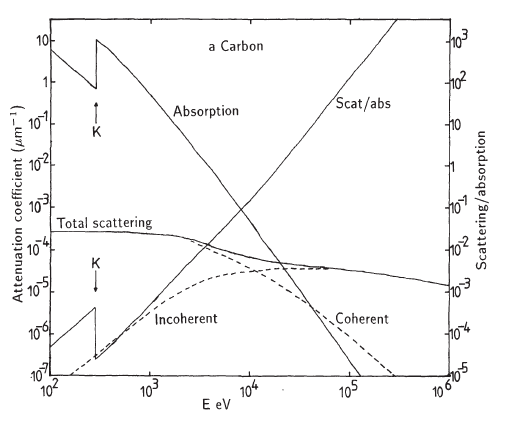
\includegraphics[width=.65\textwidth]{Immagini/Chapter1/Scattering1}}\quad
%
\subfloat[][$Pb $ \label{fig: Scattering2}]
   {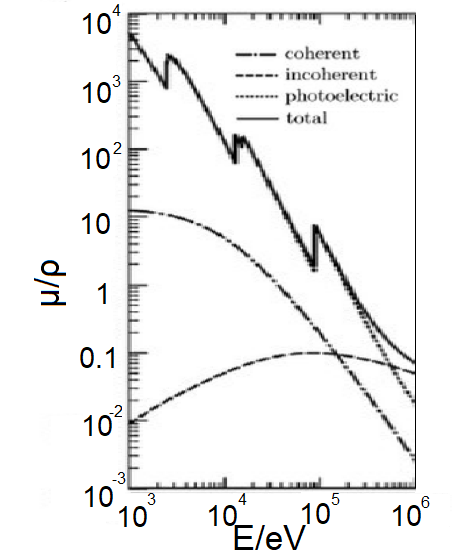
\includegraphics[width=.65\textwidth]{Immagini/Chapter1/Scattering2}}
%
\caption{Attenuation coefficient for X-ray radiation of a light material (water Figure \ref{fig: Scattering1}), and a heavy material (lead \ref{fig: Scattering2}) (from \cite{article_res_geat}).}
\label{fig :AttenuationCoefficient}
%
\end{figure}
Figure \ref{fig :AttenuationCoefficient} show the contribution for the attenuation coefficient, of the different absorption of a light material (water Figure \ref{fig: Scattering1}), and a heavy material (lead \ref{fig: Scattering2}) (from \cite{article_res_geat}.
\section{Interaction with Matter}
\label{sec: Interaction with Matter}
Interaction between radiation and matter can be compressed in a coefficient (absorption coefficient)), that rule the attenuation of an incident radiation
\begin{equation}
I = I_0 exp(-\mu x)
\label{eq: intensity}
\end{equation}
\begin{flushleft}
where $x $ is the thickness of the material, $\mu$ is the absorption coefficient, and $I_0$ the initial intensity of the beam corresponding to the intensity at $x=0$. Considering the beam as a plane wave, it is possible to express the  amplitude of the electromagnetic wave as:
\end{flushleft}
\begin{equation}
A=A_0exp(\frac{-2 \pi \beta x}{\lambda})exp(\frac{-2 \pi i ((1 - \delta)x-ct)}{\lambda})
\label{eq: amplitude}
\end{equation}
\begin{flushleft}
where $x$ is the position of the front wave, $\lambda$ correspond to the wavelength of the wave in the vacuum, $\delta $ is a number that describe the dispersive aspect of the wave-matter interaction, and $\beta $ is the absorption coefficient that describe the absorption aspect of the wave-matter interaction. The propagation of the radiation depends on the complex refractive index $n $, that can be expressed as: 
\end{flushleft}
\begin{equation}
n = 1 - \delta - i \beta
\label{eq: n_comlex}
\end{equation}
\begin{flushleft}
For X-rays process, the absorption term is the leading term, this mean that the $\mu$ coefficient can be defined as linearly dependent from the absorption coefficient, where:
\end{flushleft}
\begin{equation}
\alpha = \frac{4 \pi \beta}{\lambda}
\label{eq: alpha1}
\end{equation}
\begin{flushleft}
Normally the absorption values tabulated are given are the mass absorption coefficients $\mu_m$, where
\end{flushleft}
\begin{equation}
\mu = \mu_m \rho
\label{eq: alpha2}
\end{equation}
\begin{flushleft}
where $\rho $ is the density of the material. The mass absorption of a compound is given by
\end{flushleft}
\begin{equation}
\mu \textsubscript{m,com} = \sum_{j} w_j \mu_{m,j}
\label{eq: mu_com}
\end{equation}
\begin{flushleft}
where $\mu_{m,j} $ is the mass absorption of a particular element, and $w_j $ is the fraction of the $j $ element in the material. The relation between the absorption coefficient of the material and the mass absorption coefficient is:
\end{flushleft}
\begin{equation}
\alpha \textsubscript{com} = \mu \textsubscript{m,com} \rho \textsubscript{com}
\label{eq: alpha com}
\end{equation}
\begin{flushleft}
where $\rho \textsubscript{com}$ is the density of the compound.
\end{flushleft}
Because of the dominant energy of the radiation with respect to the matter energies involved in the interaction (X-rays energies spreads from 100eV, soft X-ray, to 10keV, hard X-ray, binding and molecular energies are of the order of few eV), the ionization process, as said before, is the leading process in the absorption coefficient. In this case the greater part of the energies involved is transferred to the kinetic term of the ionized electrons. Electron in atom have a well-defined state of energies, so, to be absorbed, the radiation must have at least an energy equal to an electron state energies. For energies equal to the electron state energies, as showed in Figure \ref{fig :AttenuationCoefficient}, absorption edges appears. The nomenclature $K,L,,M $, of those edges, that are not important for our treatment, correspond to, as it is showed in Figure \ref{fig: KLM}, the energies of an electron that goes down from a greater level, for example $n=2 $ to a lower one $n=1 $ (\cite{agarwal1991interaction}). In reality, the edges, are less pronunciation as the ones in figure, due to the finite energy width of the states, and because of the environment effect.
\\
\begin{figure}[]
%
\centering
%
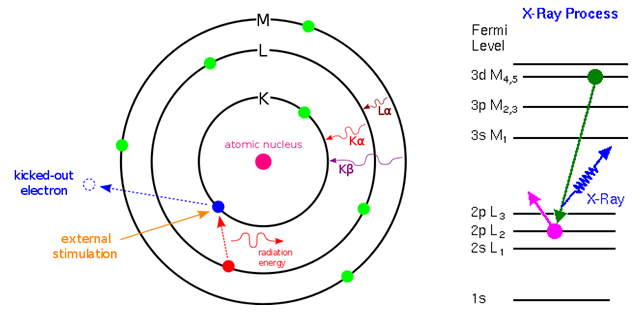
\includegraphics[width=.6\textwidth]{Immagini/Chapter1/KLM}
%
\caption{X-ray ionizing process}
%
\label{fig: KLM}
%
\end{figure}
To understand better the absorption of the X-ray radiation it is reported a brief theoretical treatment of the interaction, because the result are useful for the design of the optical element used for X-rays. The calculation start from the elastic scattering between  X-ray photon against free electron (Thomson scattering). The electro-magnetic radiation is characterized by an electric field with amplitude $A_0$ that accelerate a free electron (of charge $e $ and mass $m_e $) by an amount of $A_0 $($e / m $). A charged particle that is accelerated emits radiation, this change the value of the amplitude of the electric field equal to:
\begin{equation}
A_T(\Phi) = \frac{e}{4 \pi \epsilon_0 c^2 \vec{r}} \vec{a} \sin \Phi
\label{eq: At1}
\end{equation}
\begin{flushleft}
where $r $ is the distance from the charge, $\Phi $ correspond to the angle between the position vector \textbf{r} and acceleration vector \textbf{a}. Replacing \textbf{a} with $A_0 $($e / m $):
\end{flushleft}
\begin{equation}
A_T(\Phi) = A_0 \frac{e^2}{4 \pi \epsilon_0 c^2 \vec{r}} \sin \Phi
\label{eq: At2}
\end{equation}
\begin{flushleft}
To treat the interaction between the bounded electron and the radiation, going beyond the Thomson scattering, it is possible to multiply the Thomson amplitude $A_T (\Phi) $ to a complex number  $f = f_1 + if_2 $ named complex atomic scattering. Thus:
\end{flushleft}
\begin{equation}
A(\Phi, E) = A_t(\Phi) * f(E) = A_T(\Phi) [f_1(E) + if_2(E)]
\label{eq: A(fi, E)}
\end{equation}
\begin{flushleft}
where the two function $f_1 $ and $f_2 $, depend on the energy of the incident X-ray radiation that, to a first approximation, are independent of the angle between the incident and the scattered radiation $\theta $. This approximation has sense because the typical radiation length ($\sim 0.1-10nm $) is much larger than the typical length of the atomic electronic distribution ($\sim 1-50pm $), the consequence of this approximation is the possibility to consider a phase scattering of the atomic wave function. The values of the two function  $f_1 $ and $f_2 $ are calculated in the relativistic quantum dispersion theory \cite{cromer1970relativistic} and are given by:
\end{flushleft}
\begin{equation}
f_1(E) = Z + 4 \frac{\epsilon_0 m_e c}{h e^2} \int_{0}^{+ \infty}\frac{W^2 \sigma(W)}{E^2 - W^2} dW - \Delta_{rel}
\label{eq: f1}
\end{equation}
\begin{flushleft}
and
\end{flushleft}
\begin{equation}
f_2(E) = 2 \frac{\epsilon_0 m_e c}{h} E \sigma(E)
\label{eq: f2}
\end{equation}
\begin{flushleft}
In Equation \ref{eq: f1}, the first term correspond to the Thomson scattering, where $Z $ correspond to the atomic number of the atom. To add the angle-dependence of the scattering it is used the factor:
\end{flushleft}
\begin{equation}
f_0 = \int_{0}^{+ \infty} U(r) sinc \left[ \frac{4 \pi r}{\lambda} \sin \frac{\theta}{2} \right] dr
\label{f0}
\end{equation}
\begin{flushleft}
where $U(r) $ represent the radial charge distribution and $sinc(x)$ is the cardinal sine function $ = \frac{\sin x}{x} $. Considering a wavelength $\lambda $ of the order of nanometres, if $\sin \frac{\theta}{2} \leq \frac{\lambda}{2}, f_0=Z $, otherwise for $\sin \frac{\theta}{2}=\lambda$, typically, for most element $ f_0 \simeq 0.9Z $.
\end{flushleft}
In Equation \ref{eq: f1}, the second term (the anomalous dispersion integral), represent the oscillation of the electron after the interaction with the radiation, this can be obtained treating the semi-classically the problem. This approach neglects the damping, so, near the absorption edges $f1 $ is inaccurate. The second term of the Equation \ref{eq: f1}, and in Equation \ref{eq: f2} contain $\sigma $ that is the photo ionization cross section expressed in $m^2 atom ^{-1} $, a coefficient that is related to the mass absorption coefficient in this way: 
\begin{equation}
\sigma(E) = A \frac{\mu}{N_0}
\label{eq: sigma}
\end{equation}
\begin{flushleft}
where $A $ is the atomic weight and $N_0 $ the Avogadro's number ($N_0 = 6.22  10^{23} particle mol^{-1}) $. The value of $\sigma(E) $ is theoretically obtained knowing the atomic wave function of the atom, so, only for hydrogen it possible to have the correct value, for all the other system, the calculation can be done with approximation methods that give some uncertainty on $\sigma(E) $, consequently on the value of $f_1 $ and $f_2 $.
\end{flushleft}
In Equation \ref{eq: f1} the third term take in account the relativistic effect. This correction is given by \cite{cromer1970relativistic}:
\begin{equation}
\Delta_{rel} = \frac{5}{3} \frac{|E_{tot}|}{m_e c^2} + \frac{Z}{2} \left( \frac{E}{m_e c^2} \right)^2
\label{eq: Delta_rel}
\end{equation}
\begin{flushleft}
where $|E_{tot} |$ is the modulus of the total energy of the atom (that is negative), moreover, this third term is the less relevant in Equation \ref{eq: f1}, for X-ray energies, so it is possible to neglect it in the calculation.
\\
For photo absorption event by an electron bounded to an atom, far from the absorption edges, a good approximation is to consider the solid state environment distorted by the ionization of the electrons, because, the most affected electrons are the outer ones. After some calculation, is possible to relate the factors $f_1 $ and $f_2 $ with the macroscopic parameters $n $ and $\beta $:
\end{flushleft}
\begin{equation}
\delta = 1 - n = \frac{e^2 \hbar^2}{2 \epsilon_0 m_e E^2} \overline{f_1}
\label{eq: delta}
\end{equation}
\begin{flushleft}
and
\end{flushleft}
\begin{equation}
\beta = \frac{e^2 \hbar^2}{2 \epsilon_0 m_e E^2} \overline{f_2}
\label{eq: beta}
\end{equation}
\begin{flushleft}
where $\overline{f_1} $ and $\overline{f_2} $ are defined as follow:
\end{flushleft}
\begin{equation}
\overline{f_1} = \sum_j N_j f_{1j} \qquad \overline{f_2} = \sum_j N_j f_{2j}
\label{f1, f2, mean}
\end{equation}
\begin{flushleft}
and represent the average scattering factor per unit volume, $N_j $ is the total number of the particular $j $ element per unit volume. Putting everything together Equation \ref{eq: delta}, apart near the absorption edges, can be expressed as:
\end{flushleft}
\begin{equation}
\delta = \frac{N e^2 \hbar^2}{2 \epsilon_0 m_e  E^2} \overline{f_1}  = \frac{N e^2 \lambda^2}{8 \pi^2 \epsilon_0 m_e c^2} \overline{f_1}
\label{eq: delta new}
\end{equation}



\begin{flushleft}

where $N $ is the number of electrons per unit volume. For X-ray energies the value of $\delta $ is small (typically $\sim 10^{-3} $) and positive, this is important because it means that, for X-rays, the refractive index is a bit less than $1 $. It is possible to find the tabulated values of $f_1 $ and $f_2 $, \cite{henke1981atomic}, that are the main ingredient to calculate the curve in Figure \ref{fig :AttenuationCoefficient}  and these were used to generate Figure 1. This values, according to the experimental results, allow writing, far from absorption edges, the absorption coefficient $\beta $ such as:
\end{flushleft}
\begin{equation}
\beta \sim Z^2 \lambda^3
\label{eq: new beta}
\end{equation}
\begin{flushleft}
This mean that increasing the photon energy, the absorption decrease, and is it consistent with Figure \ref{fig :AttenuationCoefficient}, far from the edges. Moreover, the absorption, become bigger with the element used in the optical element, heavy elements absorb more than light elements. This is the reason why, to use refractive lenses for x-ray radiation, one of the used material is the Beryllium.
\end{flushleft}
\section{Total External Reflection}
\label{sec: Total Externa Reflection}
\begin{flushleft}
For the system in Figure \ref{fig: System}, there are two complex refractive indexes:
\end{flushleft}
\begin{equation}
\overline{n_1} = 1 - \delta_1 - i \beta_1 = n_1 - i \beta_1
\label{eq: n1}
\end{equation}
and
\begin{equation}
\overline{n_2} = 1 - \delta_2 - i \beta_2 = n_2 - i \beta_2
\label{eq: n1}
\end{equation}
\begin{flushleft}
moreover $\delta_2 > \delta_1 $. In the general case there are, as shown in Figure \ref{fig: System} a reflected and a transmitted wave. For the theoretical treatment, initially, will be neglect the absorption ($\beta_1 = \beta_2 = 0$), moreover the permeability coefficient it is supposed to be similar to the permeability in the vacuum. Thus, the law of Snell, can be expressed such as: 
\end{flushleft}
\begin{equation}
\frac{\cos \theta_i}{\cos \theta_t} = \frac{1 - \delta_2}{1 - \delta_1}
\label{eq: snell 1}
\end{equation}
\begin{figure}[]
%
\centering
%
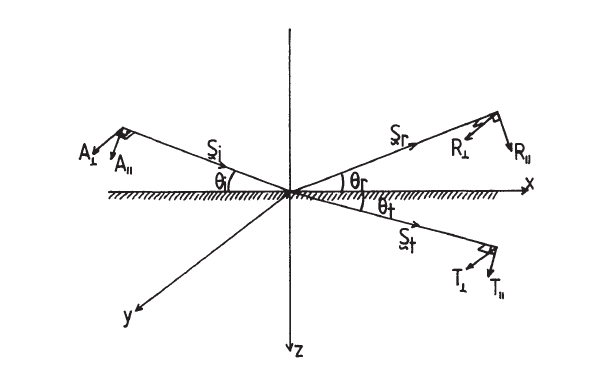
\includegraphics[width=.6\textwidth]{Immagini/Chapter1/System}
%
\caption{Interface of two medium}
%
\label{fig: System}
%
\end{figure}
\begin{flushleft}
Using the frame system as in Figure \ref{fig: System}, with the z-axis that correspond to the normal of the interface. It is possible to write the component of the electric field of the waves in this way
\end{flushleft}
\begin{subequations}
\begin{equation}
E_{ix} = A_{\parallel} \sin \theta_i \exp^{- i \tau_i}, \hspace{4mm}
E_{iy} = A_{\perp} \exp^{- i \tau_i}, \hspace{4mm} 
E_{iz} = A_{\parallel} \cos \theta_i \exp^{- i \tau_i}
\label{eq: E component 1}
\end{equation}
\begin{equation}
E_{tx} = - T_{\parallel} \sin \theta_t \exp^{- i \tau_t}, \hspace{4mm}
E_{ty} = T_{\perp} \exp^{- i \tau_t}, \hspace{4mm} 
E_{tz} = T_{\parallel} \cos \theta_t \exp^{- i \tau_t}
\label{eq: E component 2}
\end{equation}
\begin{equation}
E_{rx} = R_{\parallel} \sin \theta_r \exp^{- i \tau_r}, \hspace{4mm}
E_{ry} = R_{\perp} \exp^{- i \tau_r}, \hspace{4mm} 
E_{rz} = R_{\parallel} \cos \theta_r \exp^{- i \tau_r}
\label{eq: E component 3}
\end{equation}
\end{subequations}
\noindent  where
\begin{subequations}
\begin{equation}
\tau_i = \omega ( t - \frac{\vec{r} \bullet \vec{s_i} }{v_1}) = \omega \left[ t - \frac{(1 - \delta_1 ) ( x \cos \theta_i + z \sin \theta_i}{c} \right]
\label{eq: tau 1}
\end{equation}
\begin{equation}
\tau_t = \omega ( t - \frac{\vec{r} \bullet \vec{s_t} }{v_2}) = \omega \left[ t - \frac{(1 - \delta_2 ) ( x \cos \theta_t + z \sin \theta_t}{c} \right]
\label{eq: tau 2}
\end{equation}
\begin{equation}
\tau_r = \omega ( t - \frac{ \vec{r} \bullet \vec{s_r} }{v_1}) = \omega \left[ t - \frac{(1 - \delta_1 ) ( x \cos \theta_r + z \sin \theta_r}{c} \right]
\label{eq: tau 3}
\end{equation}
\end{subequations}
\begin{flushleft}
where $\omega $ is the angular frequency of the wave, and $v_1, v_2 $, correspond to the velocities of propagation that depend on the material as follows:
\end{flushleft}
\begin{equation}
v_1 = \frac{c}{1 - \delta_1}, \hspace{4mm} v_2 = \frac{c}{1 - \delta_2}
\end{equation}
\begin{flushleft}
the related magnetic field are:
\end{flushleft}
\begin{subequations}
\begin{equation}
\begin{aligned}
H_{ix} = - A_{\perp} (1 - \delta_1) \sin \theta_i \exp^{-i \tau_i}, \hspace{4mm}
H_{iy} = - A_{\parallel} (1 - \delta_1) \exp^{-i \tau_i}, \\
H_{iz} =  A_{\perp} (1 - \delta_1) \cos \theta_i \exp^{-i \tau_i}
\end{aligned}
\label{eq: H1}
\end{equation}
\begin{equation}
\begin{aligned}
H_{tx} = - T_{\perp} (1 - \delta_2) \sin \theta_t \exp^{-i \tau_t}, \hspace{4mm}
H_{ty} = - T_{\parallel} (1 - \delta_2) \exp^{-i \tau_t}, \\
H_{tz} =  T_{\perp} (1 - \delta_2) \cos \theta_t \exp^{-i \tau_t}
\end{aligned}
\label{eq: H2}
\end{equation}
\begin{equation}
\begin{aligned}
H_{rx} = - R_{\perp} (1 - \delta_1) \sin \theta_r \exp^{-i \tau_r}, \hspace{4mm}
H_{ry} = - R_{\parallel} (1 - \delta_1) \exp^{-i \tau_r}, \\
H_{rz} =  R_{\perp} (1 - \delta_1) \cos \theta_r \exp^{-i \tau_r}
\label{eq: H3}
\end{aligned}
\end{equation}
\end{subequations}
\begin{flushleft}
the boundary condition impose the continuity of the fields:
\end{flushleft}
\begin{equation}
E_{ix} + E_{rx} = E_{tx}, \hspace{4mm} E_{iy} + E_{ry} = E_{ty}
\label{eq: continuity E}
\end{equation}
\noindent and
\begin{equation}
H_{ix} + H_{rx} = H_{tx}, \hspace{4mm} H_{iy} + H_{ry} = H_{ty}
\label{eq: continuity H}
\end{equation}
\begin{flushleft}
because of Snell's laws $\theta_r = \theta_t $, so, from the Equation \ref{eq: continuity E} and Equation \ref{eq: continuity H}:
\end{flushleft}
\begin{subequations}
\begin{equation}
(A_{\parallel} - R_{\parallel}) \sin \theta_i = T_{\parallel} \sin_t
\label{eq: mix1}
\end{equation}
\begin{equation}
A_{\perp} + R_{\perp} = T_{\perp}
\label{eq: mix2}
\end{equation}
\begin{equation}
(1 - \delta_1 ) (A_{\perp} - R_{\perp}) \sin \theta_i = (1 - \delta_2) T_{\perp} \sin \theta_t
\label{eq: mix3}
\end{equation}
\begin{equation}
(1 - \delta_1) (A_{\parallel} +R_{\parallel}) = (1 - \delta_2) T_{\parallel}
\label{eq: mix4}
\end{equation}
\label{eq: mix}
\end{subequations}
\begin{flushleft}
Equations \ref{eq: mix} give a set of equations where the parallel and perpendicular component of the waves are independent. Solving that set with respect to each parallel/perpendicular component it is obtained:
\end{flushleft}
\begin{subequations}
\begin{equation}
\begin{aligned}
\frac{R_{\parallel}}{A_{\parallel}} = \left[\frac{(1 - \delta_2) \sin \theta_i - (1 - \delta_1) \sin \theta_t}{(1 - \delta_2) \sin \theta_i} + (1 - \delta_1) \sin \theta_t \right]
\end{aligned}
\label{eq: R/A parll}
\end{equation}
\begin{equation}
\begin{aligned}
\frac{R_{\perp}}{A_{\perp}} = \left[\frac{(1 - \delta_1) \sin \theta_i - (1 - \delta_2) \sin \theta_t}{(1 - \delta_1) \sin \theta_i} + (1 - \delta_2) \sin \theta_t \right]
\end{aligned}
\label{eq: R/A perp}
\end{equation}
\begin{equation}
\begin{aligned}
\frac{T_{\parallel}}{A_{\parallel}} = \frac{2(1 - \delta_1) \sin \theta_i}{(1 - \delta_2) \sin \theta_i + (1 - \delta_1) \sin \theta_t}
\end{aligned}
\label{eq: T/A parll}
\end{equation}
\begin{equation}
\begin{aligned}
\frac{T_{\perp}}{A_{\perp}} = \frac{2(1 - \delta_1) \sin \theta_i}{(1 - \delta_1) \sin \theta_i + (1 - \delta_2) \sin \theta_t}
\end{aligned}
\label{eq: T/A perp}
\end{equation}
\label{eq: parall and perp 1}
\end{subequations}
\begin{flushleft}
Equations \ref{eq: parall and perp 1} are the \textbf{Fresnel formula} for reflection at a plane surface. Combining them with Equation \ref{eq: snell 1} it is obtained:
\end{flushleft}
\begin{subequations}
\begin{equation}
\begin{aligned}
\frac{R_{\parallel}}{A_{\parallel}} = \frac{(1 - \delta_2)^2 \sin \theta_i - (1 - \delta_1) \sqrt{(1 - \delta_2)^2 - (1 - \delta_1)^2 \cos^2 \theta_i}}{(1 - \delta_2)^2 \sin \theta_i +  (1 - \delta_1) \sqrt{(1 - \delta_2)^2 - (1 - \delta_1)^2 \cos^2 \theta_i}} 
\end{aligned}
\label{eq: R/A parll 1}
\end{equation}
\begin{equation}
\begin{aligned}
\frac{R_{\perp}}{A_{\perp}} = \frac{(1 - \delta_1)^2 \sin \theta_i - \sqrt{(1 - \delta_2)^2 - (1 - \delta_1)^2 \cos^2 \theta_i}}{(1 - \delta_1)^2 \sin \theta_i  +  \sqrt{(1 - \delta_2)^2 - (1 - \delta_1)^2 \cos^2 \theta_i}} 
\end{aligned}
\label{eq: R/A perp 1}
\end{equation}
\begin{equation}
\begin{aligned}
\frac{T_{\parallel}}{A_{\parallel}} = \frac{2(1 - \delta_1) (1 - \delta_2) \sin \theta_i }{(1 - \delta_2)^2 \sin \theta_i  +  (1 - \delta_2)\sqrt{(1 - \delta_2)^2 - (1 - \delta_1)^2 \cos^2 \theta_i}} 
\end{aligned}
\label{eq: T/A parll 1}
\end{equation}
\begin{equation}
\begin{aligned}
\frac{T_{\perp}}{A_{\perp}} = \frac{2(1 - \delta_1) \sin \theta_i }{(1 - \delta_1) \sin \theta_i  +  \sqrt{(1 - \delta_2)^2 - (1 - \delta_1)^2 \cos^2 \theta_i}} 
\end{aligned}
\label{eq: T/A perp 1}
\end{equation}
\label{eq: parall and per 2}
\end{subequations}
\begin{flushleft}
When $\theta_i $ is such that:
\end{flushleft}
\begin{equation}
\cos \theta_c = \frac{1 - \delta_2}{1 - \delta_1}
\label{eq: theta_c}
\end{equation}
\begin{flushleft}
that angle is named critical angle $\theta_c $, and
\end{flushleft}
\begin{equation}
\frac{R_{\parallel}}{A_{\parallel}} = \frac{R_{\perp}}{A_{\perp}}
\label{eq: R/A critical}
\end{equation}
\begin{flushleft}
this case correspond to a wave that is totally reflected. Normally the total external reflection take place at an interface light material(air/vacuum) and dense material, so $\delta_1 = 0, \delta_2 = \delta$, the equations became:
\end{flushleft}
\begin{equation}
\cos \theta_c = 1 - \delta \qquad for \hspace{2mm} small \hspace{2mm} angle \qquad \theta_c \simeq \sqrt{2 \delta}
\end{equation}
\begin{flushleft}
and:
\end{flushleft}
\begin{subequations}
\begin{equation}
\begin{aligned}
\frac{R_{\parallel}}{A_{\parallel}} = \frac{(1 - \delta)^2 \sin \theta_i - \sqrt{(1 - \delta)^2 - \cos^2 \theta_i}}{(1 - \delta)^2 \sin \theta_i + \sqrt{(1 - \delta_2)^2 - \cos^2 \theta_i}} 
\end{aligned}
\label{eq: R/A parll 2}
\end{equation}
\begin{equation}
\begin{aligned}
\frac{R_{\perp}}{A_{\perp}} = \frac{\sin \theta_i - \sqrt{(1 - \delta)^2 - (1 - \cos^2 \theta_i}}{\sin \theta_i  +  \sqrt{(1 - \delta)^2 - \cos^2 \theta_i}} 
\end{aligned}
\label{eq: R/A perp 2}
\end{equation}
\begin{equation}
\begin{aligned}
\frac{T_{\parallel}}{A_{\parallel}} = \frac{2(1 - \delta) \sin \theta_i }{(1 - \delta)^2 \sin \theta_i  +  \sqrt{(1 - \delta)^2 - (1 - \cos^2 \theta_i}} 
\end{aligned}
\label{eq: T/A parll 2}
\end{equation}
\begin{equation}
\begin{aligned}
\frac{T_{\perp}}{A_{\perp}} = \frac{2 \sin \theta_i }{ \sin \theta_i  +  \sqrt{(1 - \delta)^2 - \cos^2 \theta_i}} 
\end{aligned}
\label{eq: T/A perp 2}
\end{equation}
\label{eq: parall and per 3}
\end{subequations}
\begin{flushleft}
introducing the absorbing coefficient $\beta_2 = \beta \neq 0 $:
\end{flushleft}
\begin{subequations}
\begin{equation}
\begin{aligned}
\frac{R_{\parallel}}{A_{\parallel}} = \frac{\overline{n}^2 \sin \theta_i - \sqrt{\overline{n}^2 - \cos^2 \theta_i}}{\overline{n}^2 \sin \theta_i + \sqrt{\overline{n}^2 - \cos^2 \theta_i}} 
\end{aligned}
\label{eq: R/A parll 3}
\end{equation}
\begin{equation}
\begin{aligned}
\frac{R_{\perp}}{A_{\perp}} = \frac{\sin \theta_i - \sqrt{\overline{n}^2 - \cos^2 \theta_i}}{(\sin \theta_i  +  \sqrt{\overline{n}^2 - \cos^2 \theta_i}} 
\end{aligned}
\label{eq: R/A perp 3}
\end{equation}
\begin{equation}
\begin{aligned}
\frac{T_{\parallel}}{A_{\parallel}} = \frac{2\overline{n} \sin \theta_i }{\overline{n}^2 \sin \theta_i  +  \sqrt{\overline{n}^2 - \cos^2 \theta_i}} 
\end{aligned}
\label{eq: T/A parll 3}
\end{equation}
\begin{equation}
\begin{aligned}
\frac{T_{\perp}}{A_{\perp}} = \frac{2 \sin \theta_i }{ \sin \theta_i  +  \sqrt{\overline{n}^2 - \cos^2 \theta_i}} 
\end{aligned}
\label{eq: T/A perp 3}
\end{equation}
\label{eq: parall and per 4}
\end{subequations}
For interface that are curved, the Equations \ref{eq: parall and per 4} are still valid if the curvature radius is much grater that the wavelength, condition that is satisfied for the X-ray radiation.
The reflectivity are defined in this way:
\begin{equation}
R_p =\frac{R_{\parallel}}{A_{\parallel}} \left(\frac{R_{\parallel}}{A_{\parallel}} \right)^{*}
\label{eq: Rp}
\end{equation}
\noindent and
\begin{equation}
R_p =\frac{R_{\parallel}}{A_{\parallel}} \left(\frac{R_{\parallel}}{A_{\parallel}} \right)^{*}
\label{eq: Rs}
\end{equation}
\begin{flushleft}
Figure \ref{fig: IdealReflection}, show the behaviour of an ideal non absorbing material ($\beta = 0 $), where the reflection maintain its initial value up to the critical angle, and after fall down, in a way ruled by the dispersion coefficient $\delta $ which depend on the energy. In reality $\beta $ is never zero, so it is not possible to have total external reflection in the way defined before. It is convenient to define that the total external appear when there is  a point of inflection in the reflection curve with respect to the incidence angle $\theta_i $, this occurs when:
\end{flushleft}
\begin{equation}
\beta < 0.63 \delta
\label{eq: last}
\end{equation}
\begin{flushleft}
In Figure \ref{fig : Plottts} are plotted the reflectivity trend of three material (Si, Rh, Pb) with respect to the incidence angle, fixing the energy of the radiation at $5000 eV$, on a silicon substrate. As it is figured there is a  better behaviour, in sense of critical angle, for the light element because of them minor absorption coefficient $\beta $. This dependant mirror reflectivity is not implemented in my python library MONWES (but it could be done). 
\end{flushleft}
\begin{figure}[]
%
\centering
%
\subfloat[][Reflectivity for the case of a non-absorbing material \label{fig: IdealReflection}]
   {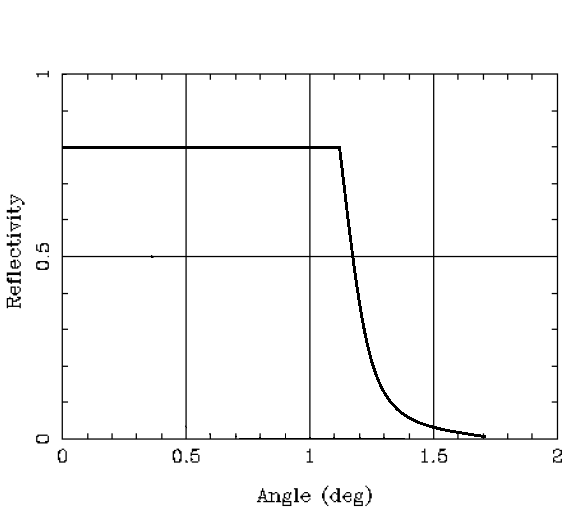
\includegraphics[width=.55\textwidth]{Immagini/Chapter1/IdealReflection}}
%
\subfloat[][Si  \label{fig: Si}]
   {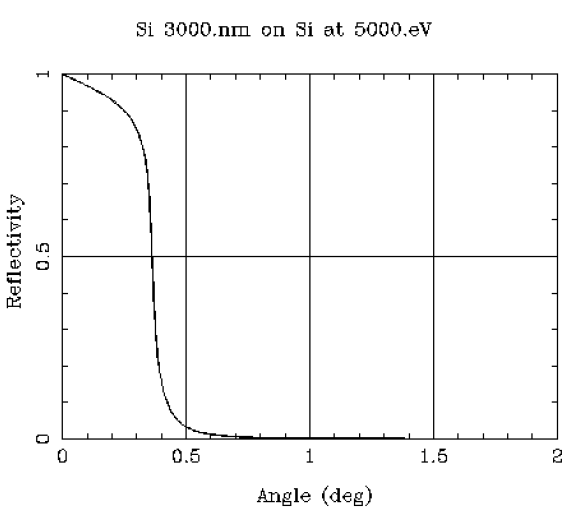
\includegraphics[width=.55\textwidth]{Immagini/Chapter1/Si}}\quad
%
\subfloat[][Rh \label{fig: Rh}]
   {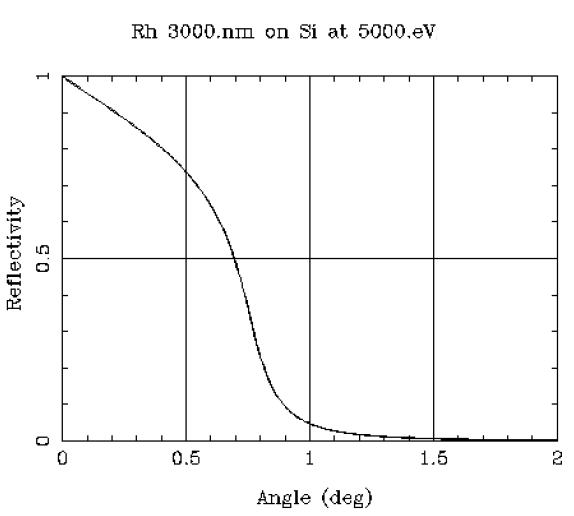
\includegraphics[width=.55\textwidth]{Immagini/Chapter1/Rh}}
%
\subfloat[][Pb  \label{fig: Si}]
   {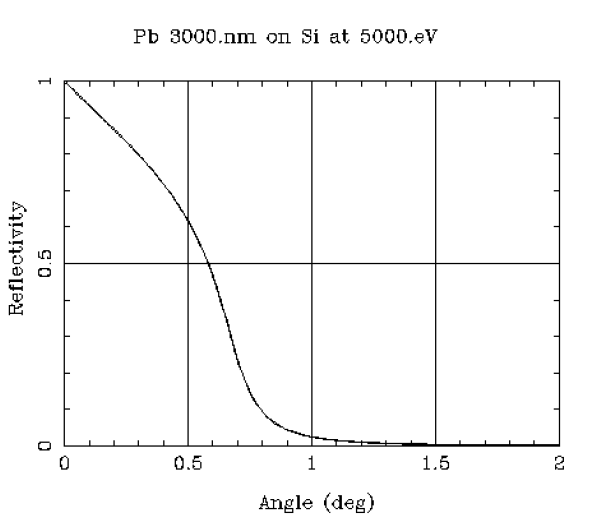
\includegraphics[width=.55\textwidth]{Immagini/Chapter1/Pb}}
%
\caption{Reflectivity plot with respect of the grazing incidence angle $\theta_i $ of different material with a radiation of $500 eV$ on a substrate of Si \cite{CXRO}. It is also plotted the behaviour of an ideal non-absorbing material \ref{fig: IdealReflection}}
\label{fig : Plottts}
%
\end{figure}